% answers.tex —— 2006 年·普通高等学校招生考试·陕西卷文科 · 参考答案与详细解析片段
% 由 tools/generate_projects.py 依来源总账自 2006/2006_数学真题_陕西文_试题.md + 2006/2006_数学真题_陕西文_解析正文.md + 2006/2006_数学真题_陕西文_答案要点.md 生成，勿手改（改源 MD 后重跑）


\begin{gktip}
固定候选 PDF 仅见题面，未见答案、解析或评分材料。以下为据固定题面独立推导并经过独立数学复核的非官方解析正文；发布者、版次、来源链和官方身份未核。题面条件或措辞存在未决项时，在对应题内保留 U/PENDING；试卷 ID 已登记，官方答案字段保持空值。
\end{gktip}

\begin{answer}
\gksolhead{1}{}

\textbf{题目}：

已知集合 \(P=\{x\in\mathbb N\mid 1\le x\le10\}\)，集合 \(Q=\{x\in\mathbb R\mid x^2+x-6=0\}\)，则 \(P\cap Q\) 等于（ ）。

(A) \(\{2\}\)　(B) \(\{3\}\)　(C) \(\{-2,3\}\)　(D) \(\{-3,2\}\)

\Needspace{4\baselineskip}
\textbf{解析}

由 $x^2+x-6=(x+3)(x-2)$，实数解为 $-3,2$。集合 $P$ 只含 $1$ 到 $10$ 的自然数，因此与 $P$ 的交集为 ${2}$，对应选项 A。

\gkanswer{答案：A，{2}。}

\end{answer}
\begin{answer}
\gksolhead{2}{}

\textbf{题目}：

函数 \(f(x)=\dfrac{1}{1+x^2}\)（\(x\in\mathbb R\)）的值域是（ ）。

(A) \((0,1)\)　(B) \((0,1]\)　(C) \([0,1)\)　(D) \([0,1]\)

\Needspace{4\baselineskip}
\textbf{解析}

对任意实数 $x$，有 $1+x^2\ge1$，故 $0<f(x)\le1$。当 $x=0$ 时取到 $1$；当 $|x|\to\infty$ 时 $f(x)\to0$，但任何有限 $x$ 都不能使分母无穷大而取到 $0$。值域为 $(0,1]$，对应 B。

\gkanswer{答案：B，(0,1]。}

\end{answer}
\begin{answer}
\gksolhead{3}{}

\textbf{题目}：

已知等差数列 \(\{a_n\}\) 中，\(a_1+a_8=8\)，则该数列前 9 项和 \(S_9\) 等于（ ）。

(A) 18　(B) 27　(C) 36　(D) 45

\Needspace{4\baselineskip}
\textbf{解析}

\Needspace{5\baselineskip}
\textbf{U/PENDING：} 设等差数列首项为 $a_1$、公差为 $d$，则 $a_8=a_1+7d$。题设只给出 $2a_1+7d=8$，而
\nopagebreak[4]
\[
S_9=\frac{9}{2}(2a_1+8d)=36+\frac{9d}{2}.
\]
右式仍随 $d$ 改变。比如 $(a_1,d)=(4,0)$ 满足题设且 $S_9=36$；$(a_1,d)=(\tfrac12,1)$ 也满足题设且 $S_9=\tfrac{81}{2}$。所以题面条件不足以唯一确定 $S_9$，不能从给定选项中确定唯一答案。

\gkanswer{答案：U/PENDING。}

\end{answer}
\begin{answer}
\gksolhead{4}{}

\textbf{题目}：

设函数 \(f(x)=\log_a(x+b)\)（$a>0\text{，}a\ne1$）的图象过点 \((0,0)\)，其反函数的图象过点 \((1,2)\)，则 \(a+b\) 等于（ ）。

(A) 6　(B) 5　(C) 4　(D) 3

\Needspace{4\baselineskip}
\textbf{解析}

图象经过 $(0,0)$ 给出 $0=\log_a b$，故 $b=1$。若反函数图象经过 $(1,2)$，原函数图象就经过交换坐标所得的 $(2,1)$，所以 $1=\log_a(2+b)=\log_a3$，从而 $a=3$。于是 $a+b=4$，对应 C。

\gkanswer{答案：C，4。}

\end{answer}
\begin{answer}
\gksolhead{5}{}

\textbf{题目}：

设直线过点 \((0,a)\)，其斜率为 1，且与圆 \(x^2+y^2=2\) 相切，则 \(a\) 的值为（ ）。

(A) \(\pm\sqrt2\)　(B) \(\pm2\)　(C) \(\pm2\sqrt2\)　(D) \(\pm4\)

\Needspace{4\baselineskip}
\textbf{解析}

\Needspace{5\baselineskip}
斜率为 $1$ 且经过 $(0,a)$ 的直线为 $y=x+a$，即 $x-y+a=0$。圆心是原点，半径为 $\sqrt2$。相切条件是圆心到直线的距离等于半径：
\nopagebreak[4]
\[
\frac{|a|}{\sqrt{1^2+(-1)^2}}=\sqrt2,
\]
所以 $|a|=2$，即 $a=\pm2$，对应 B。

\gkanswer{答案：B，±2。}

\end{answer}
\begin{answer}
\gksolhead{6}{}

\textbf{题目}：

“$\alpha\text{，}\beta\text{，}\gamma$ 成等差数列”是“等式 \(\sin(\alpha+\gamma)=\sin2\beta\) 成立”的（ ）。

(A) 充分而不必要条件　(B) 必要而不充分条件
(C) 充分必要条件　(D) 既不充分也不必要条件

\Needspace{4\baselineskip}
\textbf{解析}

若 $\alpha,\beta,\gamma$ 成等差数列，则 $\alpha+\gamma=2\beta$，代入即得 $\sin(\alpha+\gamma)=\sin2\beta$，所以数列条件是等式成立的充分条件。逆向不成立：取 $\alpha=0,\gamma=\pi,\beta=0$，两边分别为 $\sin\pi=0$ 与 $\sin0=0$，但 $\alpha+\gamma=\pi\ne0=2\beta$，三数不成等差数列。故为充分而不必要条件，对应 A。

\gkanswer{答案：A，充分而不必要。}

\end{answer}
\begin{answer}
\gksolhead{7}{}

\textbf{题目}：

设 $x\text{，}y$ 为正数，则 \((x+y)\left(\dfrac1x+\dfrac4y\right)\) 的最小值为（ ）。

(A) 6　(B) 9　(C) 12　(D) 15

\Needspace{4\baselineskip}
\textbf{解析}

\Needspace{5\baselineskip}
展开并应用正数的均值不等式：
\nopagebreak[4]
\[
(x+y)\left(\frac1x+\frac4y\right)=5+\frac{x}{y}+\frac{4y}{x}\ge5+2\sqrt{\frac{x}{y}\frac{4y}{x}}=9.
\]
当 $x/y=4y/x$，即 $x=2y$ 时取等号（例如 $x=2,y=1$），故最小值是 $9$，对应 B。

\gkanswer{答案：B，9。}

\end{answer}
\begin{answer}
\gksolhead{8}{}

\textbf{题目}：

\Needspace{5\baselineskip}
已知非零向量 \(\overrightarrow{AB}\) 与 \(\overrightarrow{AC}\) 满足
\nopagebreak[4]
\[
\left(\frac{\overrightarrow{AB}}{|\overrightarrow{AB}|}+\frac{\overrightarrow{AC}}{|\overrightarrow{AC}|}\right)\cdot\overrightarrow{BC}=0
\quad\text{\text{且}}\quad
\frac{\overrightarrow{AB}}{|\overrightarrow{AB}|}\cdot\frac{\overrightarrow{AC}}{|\overrightarrow{AC}|}=\frac12\text{，}
\]
则 \(\triangle ABC\) 为（ ）。

(A) 三边均不相等的三角形　(B) 直角三角形
(C) 等腰非等边三角形　(D) 等边三角形

\Needspace{4\baselineskip}
\textbf{解析}

\Needspace{5\baselineskip}
记 $\mathbf u=\overrightarrow{AB}/|AB|$、$\mathbf v=\overrightarrow{AC}/|AC|$，并记 $|AB|=c$、$|AC|=b$。因为 $\overrightarrow{BC}=b\mathbf v-c\mathbf u$，第一条件化为
\nopagebreak[4]
\[
(\mathbf u+\mathbf v)\cdot(b\mathbf v-c\mathbf u)=(b-c)(1+\mathbf u\cdot\mathbf v)=0.
\]
第二条件给 $\mathbf u\cdot\mathbf v=\tfrac12$，所以括号第二因子为 $\tfrac32\ne0$，从而 $b=c$。两边夹角 $\theta$ 满足 $\cos\theta=\tfrac12$，故 $\theta=60^\circ$。由两边相等及夹角 $60^\circ$，第三边也等于这两边，三角形为等边三角形，对应 D。

\gkanswer{答案：D，等边三角形。}

\end{answer}
\begin{answer}
\gksolhead{9}{}

\textbf{题目}：

已知函数 \(f(x)=ax^2+2ax+4\)（\(a>0\)）。若 $x_1<x_2\text{，}x_1+x_2=0$，则（ ）。

(A) \(f(x_1)<f(x_2)\)　(B) \(f(x_1)=f(x_2)\)
(C) \(f(x_1)>f(x_2)\)　(D) \(f(x_1)\) 与 \(f(x_2)\) 的大小不能确定

\Needspace{4\baselineskip}
\textbf{解析}

\Needspace{5\baselineskip}
配方得 $f(x)=a(x+1)^2+4-a$，对称轴为 $x=-1$。条件 $x_1+x_2=0$ 表明 $x_1,x_2$ 关于 $0$ 对称，并非关于 $-1$ 对称；但直接相减可得
\nopagebreak[4]
\[
f(x_1)-f(x_2)=a(x_1-x_2)(x_1+x_2+2)=2a(x_1-x_2)<0,
\]
因为 $a>0$ 且 $x_1<x_2$。所以 $f(x_1)<f(x_2)$，对应 A。

\gkanswer{答案：A，$f(x_1)<f(x_2)$。}

\end{answer}
\begin{answer}
\gksolhead{10}{}

\textbf{题目}：

已知双曲线 \(\dfrac{x^2}{a^2}-\dfrac{y^2}{2}=1\)（\(a>\sqrt2\)）的两条渐近线的夹角为 \(\dfrac\pi3\)，则双曲线的离心率为（ ）。

(A) 2　(B) \(\sqrt3\)　(C) \(\dfrac{2\sqrt6}{3}\)　(D) \(\dfrac{2\sqrt3}{3}\)

\Needspace{4\baselineskip}
\textbf{解析}

渐近线为 $y=\pm(\sqrt2/a)x$。令其与正 $x$ 轴的锐角为 $\theta$，则两渐近线的锐夹角为 $2\theta=\pi/3$，从而斜率绝对值 $\tan\theta=1/\sqrt3=\sqrt2/a$，得 $a=\sqrt6$。双曲线的 $b^2=2$，故 $c^2=a^2+b^2=8$，离心率 $e=c/a=\sqrt8/\sqrt6=2\sqrt3/3$，对应 D。

\gkanswer{答案：D，2√3/3。}

\end{answer}
\begin{answer}
\gksolhead{11}{}

\textbf{题目}：

已知平面 \(\alpha\) 外不共线的三点 $A\text{，}B\text{，}C$ 到 \(\alpha\) 的距离都相等，则正确的结论是（ ）。

(A) 平面 \(ABC\) 必平行于 \(\alpha\)
(B) 平面 \(ABC\) 必与 \(\alpha\) 相交
(C) 平面 \(ABC\) 必不垂直于 \(\alpha\)
(D) 存在 \(\triangle ABC\) 的一条中位线平行于 \(\alpha\) 或在 \(\alpha\) 内

\Needspace{4\baselineskip}
\textbf{解析}

取 $\alpha$ 为 $z=0$ 平面。三点到该平面的距离相等，意味着三点的有向 $z$ 坐标只能是同一个常数 $h$，或分别取 $h$ 与 $-h$（这里 $h>0$）。若同侧，则三点都在平面 $z=h$ 或 $z=-h$ 上，故 $ABC$ 所在平面平行于 $\alpha$；其任一中位线平行于 $\alpha$。

若有两点在一侧、另一点在另一侧，不妨设 $A,B$ 的高度为 $h$，$C$ 的高度为 $-h$。边 $AC$ 与 $BC$ 的中点均在 $z=0$ 平面内。连接 $AC$、$BC$ 中点的三角形中位线平行于 $AB$，而 $AB$ 平行于 $\alpha$，因此这条中位线也平行于 $\alpha$。交换两侧的点也同理。故 D 必成立。

\gkanswer{答案：D。}

\end{answer}
\begin{answer}
\gksolhead{12}{}

\textbf{题目}：

为确保信息安全，信息需加密传播，发送方由明文 \(\to\) 密文（加密），接收方由密文 \(\to\) 明文（解密）。已知加密规则为：明文 $a\text{，}b\text{，}c\text{，}d$ 对应密文 $a+2b\text{，}2b+c\text{，}2c+3d\text{，}4d$。例如，明文 1，2，3，4 对应密文 5，7，18，16。当接收方收到密文 14，9，23，28 时，则解密得到的明文为（ ）。

(A) 1，6，4，7　(B) 4，6，1，7　(C) 7，6，1，4　(D) 6，4，1，7

\Needspace{4\baselineskip}
\textbf{解析}

设明文为 $(a,b,c,d)$。由最后一个密文数得到 $4d=28$，故 $d=7$。第三个密文数给 $2c+3d=23$，代入 $d=7$ 得 $2c=2$、$c=1$。第二个密文数给 $2b+c=9$，所以 $b=4$；第一个给 $a+2b=14$，所以 $a=6$。明文为 $(6,4,1,7)$，对应 D。

\gkanswer{答案：D，(6,4,1,7)。}

\end{answer}
\begin{answer}
\gksolhead{13}{}

\textbf{题目}：

\(\cos43^\circ\cos77^\circ+\sin43^\circ\cos167^\circ\) 的值为 \gkblank{}。

\Needspace{4\baselineskip}
\textbf{解析}

\Needspace{5\baselineskip}
由 $\cos167^\circ=-\cos13^\circ$，原式为
\nopagebreak[4]
\[
\cos43^\circ\cos77^\circ-\sin43^\circ\cos13^\circ.
\]
\Needspace{5\baselineskip}
又 $\cos77^\circ=\sin13^\circ$，故原式
\nopagebreak[4]
\[
=\cos43^\circ\sin13^\circ-\sin43^\circ\cos13^\circ
=\sin(13^\circ-43^\circ)=-\frac12.
\]

\gkanswer{答案：$-$1/2。}

\end{answer}
\begin{answer}
\gksolhead{14}{}

\textbf{题目}：

\(\left(2x-\dfrac1{\sqrt{x}}\right)^6\) 展开式中的常数项为 \gkblank{}。（用数字作答）

\Needspace{4\baselineskip}
\textbf{解析}

\Needspace{5\baselineskip}
二项展开的第 $k+1$ 项为
\nopagebreak[4]
\[
\binom6k(2x)^{6-k}\left(-x^{-1/2}\right)^k
=\binom6k2^{6-k}(-1)^k x^{6-3k/2}.
\]
常数项要求指数 $6-\tfrac32k=0$，故 $k=4$。该项系数是 $\binom64 2^2(-1)^4=15\cdot4=60$。

\gkanswer{答案：60。}

\end{answer}
\begin{answer}
\gksolhead{15}{}

\textbf{题目}：

某校从 8 名教师中选派 4 名教师同时去 4 个边远地区支教（每地 1 人），其中甲和乙不同去，则不同的选派方案共有 \gkblank{} 种。

\begin{gktip}
原页原文“甲和乙不同去”照录；本阶段不按推测解释该选派条件。
\end{gktip}

\Needspace{4\baselineskip}
\textbf{解析}

\textbf{U/PENDING：} 固定题面写作“甲和乙不同去”，但这句话不能据现有明文唯一判断其选派关系。它可能涉及两人是否同时入选，也可能涉及分别去不同地区等含义；不同解释会改变计数集合。题面本身未消除该歧义，因此无法唯一确定方案数，本解析不按猜测补定条件。

\gkanswer{答案：U/PENDING。}

\end{answer}
\begin{answer}
\gksolhead{16}{}

\textbf{题目}：

水平桌面 \(\alpha\) 上放有 4 个半径均为 \(2R\) 的球，且相邻的球都相切（球心的连线构成正方形）。在这 4 个球的上面放 1 个半径为 \(R\) 的小球，它和下面的 4 个球恰好都相切，则小球的球心到水平桌面 \(\alpha\) 的距离是 \gkblank{}。

\Needspace{4\baselineskip}
\textbf{解析}

\Needspace{5\baselineskip}
设四个大球球心为正方形四顶点，正方形边长为 $4R$。小球球心到每个大球球心的距离均为 $R+2R=3R$；由于到四顶点等距，其在正方形平面上的投影是正方形中心。中心至任一顶点的水平距离为正方形对角线的一半，即 $2\sqrt2R$。若小球球心到该平面的垂直距离为 $h$，则
\nopagebreak[4]
\[
h^2+(2\sqrt2R)^2=(3R)^2,
\]
故 $h=R$。大球球心距桌面为 $2R$，所以小球球心距桌面为 $2R+h=3R$。

\gkanswer{答案：3R。}

\end{answer}
\begin{answer}
\gksolhead{17}{}

\textbf{题目}：

甲、乙、丙 3 人投篮，投进的概率分别是 $\dfrac25\text{，}\dfrac12\text{，}\dfrac35$。现 3 人各投篮 1 次，求：

(1) 3 人都投进的概率；
(2) 3 人中恰有 2 人投进的概率。

\Needspace{4\baselineskip}
\textbf{解析}

\gksubpart{(1) 三人都投进}

\Needspace{5\baselineskip}
三人的投篮结果相互独立，因此都投进的概率为
\nopagebreak[4]
\[
\frac25\cdot\frac12\cdot\frac35=\frac{3}{25}.
\]

\gksubpart{(2) 恰有两人投进}

\Needspace{5\baselineskip}
按未投进的人分类，三个互斥情形的概率分别为
\nopagebreak[4]
\[
\left(\frac25\cdot\frac12\cdot\frac25\right),\quad
\left(\frac25\cdot\frac12\cdot\frac35\right),\quad
\left(\frac35\cdot\frac12\cdot\frac35\right).
\]
相加得 $\frac{4}{50}+\frac{6}{50}+\frac{9}{50}=\frac{19}{50}$。

\gkanswer{答案（1）：3/25。}

\gkanswer{答案（2）：19/50。}

\end{answer}
\begin{answer}
\gksolhead{18}{}

\textbf{题目}：

已知函数 \(f(x)=\sqrt3\sin\left(2x-\dfrac\pi6\right)+2\sin^2\left(x-\dfrac\pi{12}\right)\)（\(x\in\mathbb R\)）。

(1) 求函数 \(f(x)\) 的最小正周期；
(2) 求使函数 \(f(x)\) 取得最大值的 \(x\) 的集合。

\Needspace{4\baselineskip}
\textbf{解析}

\gksubpart{(1) 最小正周期}

\Needspace{5\baselineskip}
令 $u=x-\tfrac\pi{12}$，则 $2x-\tfrac\pi6=2u$，且 $2\sin^2u=1-\cos2u$。于是
\nopagebreak[4]
\[
f(x)=1+\sqrt3\sin2u-\cos2u=1+2\sin\left(2u-\frac\pi6\right).
\]
相位中的自变量是 $2u$，故周期为 $\pi$。因正弦项系数非零，基本周期不能再缩短，最小正周期为 $\pi$。

\gksubpart{(2) 取得最大值的自变量}

\Needspace{5\baselineskip}
上式最大值在 $\sin(2u-\tfrac\pi6)=1$ 时取得，即
\nopagebreak[4]
\[
2u-\frac\pi6=\frac\pi2+2k\pi,\qquad k\in\mathbb Z.
\]
\Needspace{5\baselineskip}
所以 $u=\tfrac\pi3+k\pi$，代回 $x=u+\tfrac\pi{12}$，得
\nopagebreak[4]
\[
x=\frac{5\pi}{12}+k\pi,\qquad k\in\mathbb Z.
\]

\gkanswer{答案（1）：最小正周期 $\pi$。}

\gkanswer{答案（2）：$x=\frac{5\pi}{12}+k\pi$，$k\in\mathbb Z$。}

\end{answer}
\begin{answer}
\gksolhead{19}{}

\textbf{题目}：

如图，$\alpha\perp\beta\text{，}\alpha\cap\beta=l\text{，}A\in\alpha\text{，}B\in\beta$，点 \(A\) 在直线 \(l\) 上的射影为 \(A_1\)，点 \(B\) 在 \(l\) 上的射影为 \(B_1\)。已知 $AB=2\text{，}AA_1=1\text{，}BB_1=\sqrt2$。求：

(1) 直线 \(AB\) 分别与平面 $\alpha\text{，}\beta$ 所成角的大小；
(2) 二面角 \(A_1-AB-B_1\) 的大小。
\nopagebreak[4]
\begin{center}% Source-faithful schematic draft: src-d3bb569fc2c589e075c748b1494aaadeaae67bbe0e3926306e123e08de2a5fec
% Source SHA-256 ef53636f75f8cef48067ff22478f699a5ac7d3dee4a42f06e01e640bc906d221; PDF p.1, Q19.
% Diagram topology only; no measurements, angle, or additional incidence claims beyond visible projections.
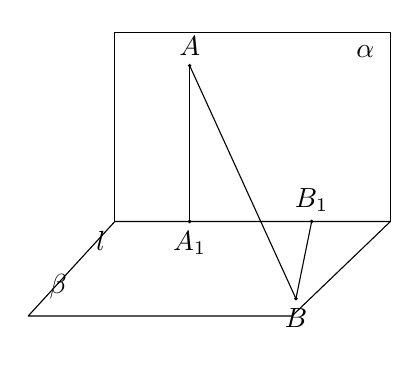
\begin{tikzpicture}[line join=round, line cap=round]
  % Plane alpha, shown as a vertical parallelogram, and its lower edge l.
  \draw (0,0) -- (3.5,0) -- (3.5,2.4) -- (0,2.4) -- cycle;
  \node at (3.18,2.16) {$\alpha$};
  % Plane beta, shown receding below l; shared edge is the intersection l.
  \draw (0,0) -- (3.5,0) -- (2.25,-1.2) -- (-1.1,-1.2) -- cycle;
  \node at (-0.72,-0.83) {$\beta$};
  \node[below left] at (0,0) {$l$};
  % A and B with their visible projections A_1 and B_1 onto l.
  \coordinate (A) at (0.95,1.98);
  \coordinate (Aone) at (0.95,0);
  \coordinate (B) at (2.30,-0.98);
  \coordinate (Bone) at (2.50,0);
  \draw (A)--(B);
  \draw (A)--(Aone);
  \draw (B)--(Bone);
  \fill (A) circle (0.7pt) node[above] {$A$};
  \fill (B) circle (0.7pt) node[below] {$B$};
  \fill (Aone) circle (0.7pt) node[below] {$A_1$};
  \fill (Bone) circle (0.7pt) node[above] {$B_1$};
\end{tikzpicture}
\end{center}
\nopagebreak[4]
\Needspace{4\baselineskip}
\textbf{解析}

\gksubpart{(1) 直线与两平面的夹角}

\Needspace{5\baselineskip}
由于 $AA_1\perp l$ 且 $BB_1\perp l$，四边形 $AA_1B_1B$ 在含 $l$ 的两个互相垂直方向上分解。具体地，$A_1B_1\subset l$，并且 $AA_1\perp l$、$BB_1\perp l$，故
\nopagebreak[4]
\[
AB^2=A_1B_1^2+AA_1^2+BB_1^2.
\]
\Needspace{5\baselineskip}
因此 $A_1B_1^2=4-1-2=1$，即 $A_1B_1=1$。直线 $AB$ 在 $\alpha$ 上的正射影为 $AA_1B_1$ 中的 $AB_1$；在 $\beta$ 上的射影为 $A_1B$。相应地，线面角 $\theta_\alpha$ 满足
\nopagebreak[4]
\[
\sin\theta_\alpha=\frac{BB_1}{AB}=\frac{\sqrt2}{2},
\]
\Needspace{5\baselineskip}
而 $\theta_\alpha=\pi/4$。线面角 $\theta_\beta$ 满足
\nopagebreak[4]
\[
\sin\theta_\beta=\frac{AA_1}{AB}=\frac12,
\]
故 $\theta_\beta=\pi/6$。

\gksubpart{(2) 二面角}

\Needspace{5\baselineskip}
取 $A_1=(0,0,0)$，以 $l$ 为 $x$ 轴、$A_1A$ 为 $y$ 轴、垂直于 $\alpha$ 的方向为 $z$ 轴。可令 $A=(0,1,0)$、$B_1=(1,0,0)$；由 $AB_1^2=AB^2-AA_1^2-BB_1^2=1$ 且 $AB_1\perp BB_1$，可取 $B=(1,0,\sqrt2)$。于是
\nopagebreak[4]
\[
\overrightarrow{AB}=(1,-1,\sqrt2),\quad
\overrightarrow{AA_1}=(0,-1,0),\quad
\overrightarrow{AB_1}=(1,-1,0).
\]
\Needspace{5\baselineskip}
二面角 $A_1-AB-B_1$ 的两个面分别为 $A_1AB$ 与 $BAB_1$。它们的法向量可分别取
\nopagebreak[4]
\[
\mathbf n_1=\overrightarrow{AB}\times\overrightarrow{AA_1}=(\sqrt2,0,-1),\qquad
\mathbf n_2=\overrightarrow{AB}\times\overrightarrow{AB_1}=(\sqrt2,\sqrt2,0).
\]
两法向量模分别为 $\sqrt3$、$2$，点积为 $2$，故两面的锐夹角余弦为 $2/(2\sqrt3)=1/\sqrt3$。因此题设二面角为 $\arccos(1/\sqrt3)$。

\gkanswer{答案（1）：直线 $AB$ 与 $\alpha$、$\beta$ 的夹角依次为 $\frac\pi4$、$\frac\pi6$。}

\gkanswer{答案（2）：arccos(1/√3)。}

\end{answer}
\begin{answer}
\gksolhead{20}{}

\textbf{题目}：

已知正项数列 \(\{a_n\}\)，其前 \(n\) 项和 \(S_n\) 满足 \(10S_n=a_n^2+5a_n+6\)，且 $a_1\text{，}a_3\text{，}a_{15}$ 成等比数列，求数列 \(\{a_n\}\) 的通项 \(a_n\)。

\Needspace{4\baselineskip}
\textbf{解析}

\Needspace{5\baselineskip}
对 $n\ge2$，将第 $n$ 项的和式与第 $n-1$ 项的和式相减：
\nopagebreak[4]
\[
10a_n=(a_n^2+5a_n+6)-(a_{n-1}^2+5a_{n-1}+6),
\]
\Needspace{5\baselineskip}
整理为
\nopagebreak[4]
\[
(a_n-a_{n-1}-5)(a_n+a_{n-1})=0.
\]
\Needspace{5\baselineskip}
数列各项为正，故 $a_n+a_{n-1}>0$，只能有 $a_n-a_{n-1}=5$。原式在 $n=1$ 时给
\nopagebreak[4]
\[
a_1^2-5a_1+6=0,
\]
所以 $a_1=2$ 或 $3$。由递推关系 $a_n=a_1+5(n-1)$，并利用 $a_1,a_3,a_{15}$ 成等比数列的条件 $a_3^2=a_1a_{15}$。若 $a_1=2$，则 $a_3=12,a_{15}=72$，满足 $12^2=2\cdot72$；若 $a_1=3$，则 $a_3=13,a_{15}=73$，但 $13^2\ne3\cdot73$。因此 $a_1=2$，通项为 $a_n=5n-3$。

\gkanswer{答案：$a_n=5n-3$。}

\end{answer}
\begin{answer}
\gksolhead{21}{}

\textbf{题目}：

\Needspace{5\baselineskip}
如图，三定点 $A(2\text{，}1)\text{，}B(0\text{，}-1)\text{，}C(-2\text{，}1)$，三动点 $D\text{，}E\text{，}M$ 满足
\nopagebreak[4]
\[
\overrightarrow{AD}=t\overrightarrow{AB}\text{，}\quad \overrightarrow{BE}=t\overrightarrow{BC}\text{，}\quad \overrightarrow{DM}=t\overrightarrow{DE}\text{，}\quad t\in[0\text{，}1]\mbox{。}
\]
(1) 求动直线 \(DE\) 斜率的变化范围；
(2) 求动点 \(M\) 的轨迹方程。
\nopagebreak[4]
\begin{center}% Source-faithful schematic draft: src-d3bb569fc2c589e075c748b1494aaadeaae67bbe0e3926306e123e08de2a5fec
% Source SHA-256 ef53636f75f8cef48067ff22478f699a5ac7d3dee4a42f06e01e640bc906d221; PDF p.2, Q21.
% Schematic parameter t=0.4 illustrates AD=t AB, BE=t BC, DM=t DE; this is not an extra value imposed by the source question.
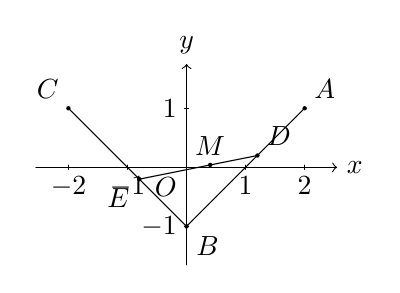
\begin{tikzpicture}[line cap=round, line join=round, x=0.75cm, y=0.75cm]
  \draw[->] (-2.55,0)--(2.55,0) node[right] {$x$};
  \draw[->] (0,-1.65)--(0,1.75) node[above] {$y$};
  \draw (-2,1)--(0,-1)--(2,1);
  \coordinate (A) at (2,1); \coordinate (B) at (0,-1); \coordinate (C) at (-2,1);
  % D and E lie on the two visible sides; M lies on the segment DE.
  \coordinate (D) at (1.2,0.2); \coordinate (E) at (-0.8,-0.2);
  \coordinate (M) at (0.4,0.04);
  \draw (D)--(E);
  \foreach \P/\label/\pos in {A/A/above right,B/B/below right,C/C/above left,D/D/above right,E/E/below left,M/M/above} {
    \fill (\P) circle (0.8pt) node[\pos] {$\label$};
  }
  \node[below left] at (0,0) {$O$};
  \node[below] at (0,-1) {};
  \foreach \xv in {-2,-1,1,2} {\draw (\xv,0.035)--(\xv,-0.035);}
  \foreach \yv in {-1,1} {\draw (0.035,\yv)--(-0.035,\yv);}
  \node[below] at (-2,0) {$-2$}; \node[below] at (-1,0) {$-1$};
  \node[below] at (1,0) {$1$}; \node[below] at (2,0) {$2$};
  \node[left] at (0,1) {$1$}; \node[left] at (0,-1) {$-1$};
\end{tikzpicture}
\end{center}
\nopagebreak[4]
\Needspace{4\baselineskip}
\textbf{解析}

\gksubpart{(1) 动直线斜率范围}

\Needspace{5\baselineskip}
由 $\overrightarrow{AB}=(-2,-2)$、$\overrightarrow{BC}=(-2,2)$，可得
\nopagebreak[4]
\[
D=A+t(B-A)=(2-2t,1-2t),\qquad E=B+t(C-B)=(-2t,-1+2t).
\]
因此 $\overrightarrow{DE}=E-D=(-2, -2+4t)$，其横坐标分量恒为 $-2\ne0$，直线斜率为 $(-2+4t)/(-2)=1-2t$。当 $t\in[0,1]$ 时，斜率范围为 $[-1,1]$。

\gksubpart{(2) 动点轨迹}

\Needspace{5\baselineskip}
由 $M=D+t(E-D)$ 得
\nopagebreak[4]
\[
M=(2-2t,1-2t)+t(-2,-2+4t)=(2-4t,1-4t+4t^2).
\]
\Needspace{5\baselineskip}
令 $x=2-4t$，则 $t=(2-x)/4$，且 $t\in[0,1]$ 等价于 $-2\le x\le2$。代入纵坐标：
\nopagebreak[4]
\[
y=1-(2-x)+\frac{(2-x)^2}{4}=\frac{x^2}{4}.
\]
故轨迹是 $y=x^2/4$ 且 $-2\le x\le2$ 的弧段。

\gkanswer{答案（1）：动直线斜率范围为 [$-$1,1]。}

\gkanswer{答案（2）：$y=\frac{x^2}{4}$，$-2\le x\le2$。}

\end{answer}
\begin{answer}
\gksolhead{22}{}

\textbf{题目}：

设函数 \(f(x)=kx^3-3x^2+1\)（\(k\ge0\)）。

(1) 求函数 \(f(x)\) 的单调区间；
(2) 若函数 \(f(x)\) 的极小值大于 0，求 \(k\) 的取值范围。

\Needspace{4\baselineskip}
\textbf{解析}

\gksubpart{(1) 单调区间}

求导得 $f'(x)=3kx^2-6x=3x(kx-2)$。

当 $k=0$ 时，$f'(x)=-6x$，故在 $(-\infty,0]$ 上递增，在 $[0,+\infty)$ 上递减。

当 $k>0$ 时，导数零点为 $0$ 与 $2/k$。在 $(-\infty,0)$ 上两个因子均为负，导数为正；在 $(0,2/k)$ 上导数为负；在 $(2/k,+\infty)$ 上导数为正。因此函数分别在 $(-\infty,0]$、$[2/k,+\infty)$ 上递增，在 $[0,2/k]$ 上递减。

\gksubpart{(2) 极小值为正时的参数范围}

\Needspace{5\baselineskip}
当 $k=0$ 时，函数只有驻点 $x=0$，该点为极大值点，不存在极小值点，不能满足“极小值大于 $0$”。若 $k>0$，由单调性可知极小值在 $x=2/k$ 处取得，且
\nopagebreak[4]
\[
f\left(\frac2k\right)=k\frac{8}{k^3}-3\frac4{k^2}+1=1-\frac4{k^2}.
\]
要求该值大于零，等价于 $k^2>4$。结合 $k>0$，得到 $k>2$。

\gkanswer{答案（1）：$k=0$ 时，$f$ 在 $(-\infty,0]$ 上递增、在 $[0,+\infty)$ 上递减；$k>0$ 时，$f$ 在 $(-\infty,0]$ 与 $[2/k,+\infty)$ 上递增，在 $[0,2/k]$ 上递减。}

\gkanswer{答案（2）：$k>2$。}

\end{answer}